%%%%%%%%%%%%%%%%%%%%%%%%%%%%%%%%%%%%%%%%%%%%%%%%%%%%%%%%%%%%%%%%%%%%
%% I, the copyright holder of this work, release this work into the
%% public domain. This applies worldwide. In some countries this may
%% not be legally possible; if so: I grant anyone the right to use
%% this work for any purpose, without any conditions, unless such
%% conditions are required by law.
%%%%%%%%%%%%%%%%%%%%%%%%%%%%%%%%%%%%%%%%%%%%%%%%%%%%%%%%%%%%%%%%%%%%

\documentclass{beamer}
\usetheme[faculty=phil]{fibeamer}
\usepackage[utf8]{inputenc}
\usepackage[
  main=english
]{babel}
%% These macros specify information about the presentation
\title{Classical Black Holes} %% that will be typeset on the
\subtitle{07. Geodesics around a Rotating Black Hole} %% title page.
\author{Edward Larra\~{n}aga}
%% These additional packages are used within the document:
\usepackage{ragged2e}  % `\justifying` text
\usepackage{booktabs}  % Tables
\usepackage{tabularx}
\usepackage{tikz}      % Diagrams
\usetikzlibrary{calc, shapes, backgrounds}
\usepackage{amsmath, amssymb}
\usepackage{url}       % `\url`s
\usepackage{listings}  % Code listings
\usepackage{siunitx}
\frenchspacing
\begin{document}
\frame{\maketitle}

\AtBeginSection[]{% Print an outline at the beginning of sections
\begin{frame}<beamer>
\frametitle{Outline for Part \thesection}
\tableofcontents[currentsection]
\end{frame}}

\section{Particle Motion around a Black Hole}
\begin{frame}
\Huge
Particle Motion around a Black Hole
\end{frame}

\subsection{Lagrangian Formulation}
\begin{frame}
	\huge
    Lagrangian Formulation
\end{frame}

\begin{frame}{Lagrangian Formulation}
	Stationary and axis-symmetric spacetime
	$$ ds^2 = g_{tt} dt^2 + 2g_{t \varphi} dt d\varphi + g_{rr} dr^2 + g_{\theta \theta} d\theta^2 + g_{\varphi \varphi} d\varphi^2 $$
	\pause
	Lagrangian for a particle moving in a spacetime defined by the metric $g_{\mu\nu}$
	$$ \mathcal{L} = \frac{1}{2} g_{\mu\nu} \dot{x}^\mu \dot{x}^\nu $$
	\pause
	$$ \dot{x}^\mu = \frac{dx^\mu}{d\lambda} $$
\end{frame}

\begin{frame}{Lagrangian Formulation}
	$$ \mathcal{L} = \frac{1}{2} g_{\mu\nu} \dot{x}^\mu \dot{x}^\nu = \frac{1}{2}  \left( \frac{ds}{d\lambda} \right)^2 $$
	\pause	
	$$ \mathcal{L} =\frac{1}{2} \left[ g_{tt} \dot{t}^2 + 2g_{t \varphi} \dot{t} \dot{\varphi} + g_{rr} \dot{r}^2 + g_{\theta \theta} \dot{\theta}^2 + g_{\varphi \varphi} \dot{\varphi}^2 \right] = \frac{1}{2} \delta$$
	\pause
	\[	\delta = 
	\begin{cases}
	0   &\textrm{for photons} \\
	-1  &\textrm{for massive particles}
	\end{cases}	
	\]
\end{frame}

\subsection{Conserved Quantities}
\begin{frame}
	\huge
    Conserved Quantities
\end{frame}

\begin{frame}{Conserved Quantities}	
	$$ \mathcal{L} =\frac{1}{2}  \left[ g_{tt} \dot{t}^2 + 2g_{t \varphi} \dot{t} \dot{\varphi} + g_{rr} \dot{r}^2 + g_{\theta \theta} \dot{\theta}^2 + g_{\varphi \varphi} \dot{\varphi}^2 \right] = \frac{1}{2} \delta$$
	\pause
	\begin{align*}
	p_t &= \frac{\partial \mathcal{L}}{\partial \dot{t}} =  \left[ g_{tt} \dot{t} + g_{t \varphi} \dot{\varphi} \right] = - \varepsilon  \\
	p_\varphi &= \frac{\partial \mathcal{L}}{\partial \dot{\varphi}} = \left[ g_{t \varphi} \dot{t} + g_{\varphi \varphi} \dot{\varphi} \right] = \ell_z 
	\end{align*}
\end{frame}

\begin{frame}{Conserved Quantities}
	\begin{align*}
	\varepsilon &= \frac{E}{m_0} = - g_{tt} \dot{t} - g_{t \varphi} \dot{\varphi}    \\
	\ell_z &= \frac{L_z}{m_0} =  g_{t \varphi} \dot{t} + g_{\varphi \varphi} \dot{\varphi}  
	\end{align*}
\end{frame}

\begin{frame}{Conserved Quantities}
	\begin{align*}
	\dot{t} &= \frac{\varepsilon g_{\varphi \varphi} + \ell_z g_{t \varphi}}{g_{t \varphi}^2 - g_{tt} g_{\varphi \varphi}} \\
	\dot{\varphi} &= - \frac{\varepsilon g_{t \varphi} + \ell_z g_{tt}}{g_{t \varphi}^2 - g_{tt} g_{\varphi \varphi}}  
	\end{align*}	
\end{frame}

\subsection{Effective Potential}
\begin{frame}
	\huge
    Effective Potential
\end{frame}

\begin{frame}{Effective Potential}
	$$ \mathcal{L} =\frac{1}{2} \left[ g_{tt} \dot{t}^2 + 2g_{t \varphi} \dot{t} \dot{\varphi} + g_{rr} \dot{r}^2 + g_{\theta \theta} \dot{\theta}^2 + g_{\varphi \varphi} \dot{\varphi}^2 \right] = \frac{1}{2} \delta$$
	\pause
	\[ g_{rr} \dot{r}^2 + g_{\theta \theta} \dot{\theta}^2 = V_{eff} (r, \theta) \]
	\pause
	\[ V_{eff} (r,\theta) = \frac{\varepsilon^2 g_{\varphi \varphi} + 2 \varepsilon \ell_z g_{t\varphi} + \ell_z^2 g_{tt} }{g_{t\varphi}^2-g_{tt} g_{\varphi\varphi}} + \delta \]
\end{frame}


\begin{frame}{Equations of Motion}
	$$\frac{d}{d\lambda} \left( \frac{\partial \mathcal{L}}{\partial \dot{x}^\alpha} \right) = \frac{\partial \mathcal{L}}{\partial x^\alpha} $$ 
	\pause
	$$\frac{d}{d\lambda} \left(  g_{\mu\alpha} \dot{x}^\mu \right) =  \frac{1}{2} \frac{\partial g_{\mu\nu}}{\partial x^\alpha} \dot{x}^\mu \dot{x}^\nu$$ 
	\pause
	$$\frac{d}{d\lambda} \left( g_{\mu\alpha} \dot{x}^\mu \right) =  \frac{1}{2} \frac{\partial g_{\mu\nu}}{\partial x^\alpha} \dot{x}^\mu \dot{x}^\nu$$ 
\end{frame}


\begin{frame}{Radial Equation of Motion}
	$$\frac{d}{d\lambda} \left( g_{\mu\alpha} \dot{x}^\mu \right) =  \frac{1}{2} \frac{\partial g_{\mu\nu}}{\partial x^\alpha} \dot{x}^\mu \dot{x}^\nu$$ 
	\pause
	$$\frac{d}{d\lambda} \left( g_{\mu r} \dot{x}^\mu \right) =  \frac{1}{2} \frac{\partial g_{\mu\nu}}{\partial r} \dot{x}^\mu \dot{x}^\nu$$
	\pause
	$$\frac{d}{d\lambda} \left( g_{rr} \dot{r} \right) =  \frac{1}{2} \left[ \partial_r g_{tt} \dot{t}^2 + 2\partial_r g_{t \varphi} \dot{t} \dot{\varphi} + \partial_r g_{rr} \dot{r}^2 + \partial_r g_{\theta \theta} \dot{\theta}^2 + \partial_r g_{\varphi \varphi} \dot{\varphi}^2 \right]$$
\end{frame}

\subsection{Equatorial Motion}
\begin{frame}
	\huge
    Equatorial Motion
\end{frame}

\begin{frame}{Effective Potential in the Equatorial Plane}
	Considering equatorial motion, $ \theta = \frac{\pi}{2} $, 
	\pause
	\[ g_{rr} \dot{r}^2 = V_{eff} (r) \]
	\pause
	\[ V_{eff} (r) = \frac{\varepsilon^2 g_{\varphi \varphi} + 2 \varepsilon \ell_z g_{t\varphi} + \ell_z^2 g_{tt} }{g_{t\varphi}^2-g_{tt} g_{\varphi\varphi}} + \delta \]
\end{frame}

\begin{frame}{Schwarzschild Effective Potential in the Equatorial Plane}
	Considering massive particles, $\delta = -1$, moving in the equatorial plane, $ \theta = \frac{\pi}{2} $, around Schwarzschild's geometry,
	\pause
	\[ \frac{1}{2} \dot{r}^2 = \frac{\varepsilon^2 -1}{2} - U_{eff} (r) \]
	\pause	
	\[ U_{eff} (r) = -\frac{M}{r} + \frac{\ell_z^2}{2r^2} - \frac{M\ell_z^2}{r^3} \]
\end{frame}

\begin{frame}{Schwarzschild Effective Potential in the Equatorial Plane}	
	\[ U_{eff} (r) = -\frac{M}{r} + \frac{\ell_z^2}{2r^2} - \frac{M\ell_z^2}{r^3} \]
	\pause
	$-\frac{M}{r}$: Newtonian Potential
	\bigskip
	\pause
	
	$\frac{\ell_z^2}{2r^2}$: Centrifugal Potential (repulsive)
	\bigskip
	\pause
	
	$- \frac{M\ell_z^2}{r^3}$: Relativistic Contribution. Responsible for the ISCO
\end{frame}

\begin{frame}{Schwarzschild Effective Potential in the Equatorial Plane}
	\begin{center}
      \begin{figure}
      	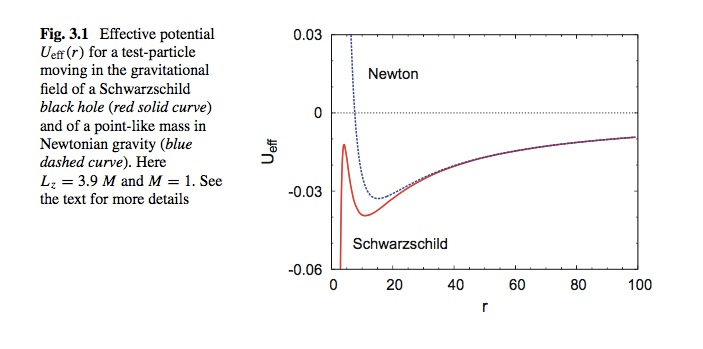
\includegraphics[scale=0.4] {figures/scheffpot.jpeg}
      \end{figure}
	\end{center}	
\end{frame}

\subsection{Equatorial Circular Orbits}
\begin{frame}
	\huge
    Equatorial Circular Orbits
\end{frame}

\begin{frame}{Circular Motion in the Equatorial Plane}
	Circular motion is obtained by the conditions
	\[ \dot{r} = \dot{\theta} = 0 \]
	\pause
	which imply
	\[ \begin{cases}
	 	&V_{eff} = 0\\
	 	&\partial_r V_{eff} = 0
	 	\end{cases} 
	 \]
\end{frame}

\begin{frame}{Equation of a Circular Motion in the Equatorial Plane}
	Another way to calculate the equation of a circular motion in the equatorial plane is taking
	$$\frac{d}{d\lambda} \left( g_{rr} \dot{r} \right) =  \frac{1}{2} \left[ \partial_r g_{tt} \dot{t}^2 + 2\partial_r g_{t \varphi} \dot{t} \dot{\varphi} + \partial_r g_{rr} \dot{r}^2 + \partial_r g_{\theta \theta} \dot{\theta}^2 + \partial_r g_{\varphi \varphi} \dot{\varphi}^2 \right]$$
	\pause
	Considering equatorial motion, $ \theta = \frac{\pi}{2} $, in circular orbits, $\ddot{r} = \dot{r} = \dot{\theta} = 0$, 	
	\pause
	$$\partial_r g_{tt} \dot{t}^2 + 2\partial_r g_{t \varphi} \dot{t} \dot{\varphi} + \partial_r g_{\varphi \varphi} \dot{\varphi}^2 =0$$
\end{frame}

\begin{frame}{Angular Velocity of a Particle in Circular Motion in the Equatorial Plane}
	$$\partial_r g_{tt} \dot{t}^2 + 2\partial_r g_{t \varphi} \dot{t} \dot{\varphi} + \partial_r g_{\varphi \varphi} \dot{\varphi}^2 =0$$
	\pause
	$$ \partial_r g_{\varphi \varphi} \left(\frac{\dot{\varphi}}{\dot{t}}\right)^2 + 2\partial_r g_{t \varphi} \left(\frac{\dot{\varphi}}{\dot{t}}\right) + \partial_r g_{tt}=0$$
	\pause
	$$\Omega =\frac{\dot{\varphi}}{\dot{t}} = \frac{-\partial_r g_{t \varphi} \pm \sqrt{\left(\partial_r g_{t \varphi}\right)^2 - \left(\partial_r g_{tt} \right) \left( \partial_r g_{\varphi \varphi}\right) ) }}{\partial_r g_{\varphi \varphi}} $$	
\end{frame}

\begin{frame}{Conserved Quantities for a Particle in Circular Motion}
	\[ \mathcal{L} =\frac{1}{2} \left[ g_{tt} \dot{t}^2 + 2g_{t \varphi} \dot{t} \dot{\varphi} + g_{rr} \dot{r}^2 + g_{\theta \theta} \dot{\theta}^2 + g_{\varphi \varphi} \dot{\varphi}^2 \right] = \frac{1}{2}  \delta \]
	\pause
	Considering $\dot{r} = \dot{\theta} = 0$, 	
	\[ \dot{t}  = \sqrt{\frac{\delta}{ g_{tt}  + 2g_{t \varphi} \Omega  + g_{\varphi \varphi} \Omega^2 }}\]
\end{frame}

\begin{frame}{Conserved Quantities for a Particle in Circular Motion}
	\[ \varepsilon = - \left( g_{tt} + \Omega g_{t\varphi} \right) \sqrt{\frac{\delta}{ g_{tt}  + 2g_{t \varphi} \Omega  + g_{\varphi \varphi} \Omega^2 }} \]
	\pause
	\[ \ell_z = - \left( g_{t\varphi} + \Omega g_{\varphi\varphi} \right) \sqrt{\frac{\delta}{ g_{tt}  + 2g_{t \varphi} \Omega  + g_{\varphi \varphi} \Omega^2 }} \]
\end{frame}

\begin{frame}{Quantities for a Particle in Circular Motion in Kerr Spacetime}
	\[ \varepsilon = \frac{r^{3/2} - 2Mr^{1/2} \pm aM^{1/2}}{r^{3/4} \sqrt{r^{3/2} - 3Mr^{1/2} \pm 2aM^{1/2}}} \]
	\pause
	\[ \ell_z = \pm \frac{M^{1/2} \left( r^2 \mp 2aM^{1/2}r^{1/2} + a^2\right) }{r^{3/4} \sqrt{r^{3/2} - 3Mr^{1/2} \pm 2aM^{1/2}}} \]
	\pause
	\[ \Omega_{\pm} = \pm \frac{M^{1/2}}{r^{3/2} \pm aM^{1/2}} \]
	\pause
	\footnotesize{Upper sign: co-rotating orbit\\ Lower sign: counter-rotating orbit}
\end{frame}


\begin{frame}{Photon Sphere}
	\[ \varepsilon = - \left( g_{tt} + \Omega g_{t\varphi} \right) \sqrt{\frac{\delta}{ g_{tt}  + 2g_{t \varphi} \Omega  + g_{\varphi \varphi} \Omega^2 }} \]
	\bigskip
	\pause
	
	For photons, $m_0 =0$. Then  $\varepsilon \rightarrow \infty$ and $\ell_z \rightarrow \infty$.\\
	\pause	
	This occurs at the  surface called \textit{phton sphere}, with radius $r = r_{ps}$ such that   
	\[ g_{tt}  + 2g_{t \varphi} \Omega  + g_{\varphi \varphi} \Omega^2 = 0 \]
\end{frame}

\begin{frame}{Photon Sphere}
	Scharzschild: $r_{ps} = 3M = \frac{3r_s}{2}$\\
	\bigskip	
	\pause
	Kerr: $r_{ps} = 2M\left\lbrace 1+ \cos\left[\frac{2}{3}\cos^{-1} \left(\mp \frac{a}{M} \right) \right] \right\rbrace $\\
	\bigskip	
	\pause
	Extreme Kerr $(M=a)$: 
	\[r_{ps} = 
	\begin{cases}
	M & \textrm{co-rotating orbit}\\
	4M & \textrm{counter-rotating orbit}
	\end{cases} \]
\end{frame}

\begin{frame}{Conserved Quantities for a Massive Particle in Circular Motion}
	Taking $\delta=-1$,
	\pause	
	\[ \varepsilon = - \left( g_{tt} + \Omega g_{t\phi} \right) \sqrt{-\frac{1}{ g_{tt}  + 2g_{t \varphi} \Omega  + g_{\varphi \varphi} \Omega^2 }} \]
	\pause
	\[ \ell_z = - \left( g_{t\varphi} + \Omega g_{\varphi\varphi} \right) \sqrt{-\frac{1}{ g_{tt}  + 2g_{t \varphi} \Omega  + g_{\varphi \phi} \Omega^2 }} \]
\end{frame}

\begin{frame}{Marginally Bound Orbit}
	For $r>r_{ps}$ not all circular orbits are bound.\\
	\pause
	Orbits with $\varepsilon \geq 1$ are unbound.\\
	\pause
	This means that giving an infinitesimal outward perturbation to a particle in this orbit, it will escape to infinity on an asymptotically hyperbolic (parabolic for the equal sign) trajectory.\\
	\pause
	The condition $\varepsilon =1$ defines the marginally bound circular orbit radius, $r=r_{mb}$.
	\pause
	\[ \varepsilon = - \left( g_{tt} + \Omega g_{t\varphi} \right) \sqrt{-\frac{1}{ g_{tt}  + 2g_{t \varphi} \Omega  + g_{\varphi \varphi} \Omega^2 }}=1 \]
\end{frame}

\begin{frame}{Marginally Bound Orbit}
	Scharzschild: $r_{mb} = 4M$\\
	\bigskip	
	\pause
	Kerr: $r_{mb} = 2M\mp a + 2\sqrt{M} \left(M \mp a \right) $\\
	\bigskip	
	\pause
	Extreme Kerr $(M=a)$: 
	\[r_{mb} = 
	\begin{cases}
	M & \textrm{co-rotating orbit}\\
	5.83M & \textrm{counter-rotating orbit}
	\end{cases} \]
\end{frame}

\begin{frame}{Marginally Stable Orbit. ISCO}
	The Marginally Stable Orbti, a.k.a. the Innermost Stable Circular Orbit (ISCO), has a radius $r=r_{ISCO}$ defined by the conditions\\
	\pause
	\begin{align*}
	\partial_r V_{eff} &= 0 \\
	\partial_r^2 V_{eff} &= 0
	\end{align*}	 
	Circular orbits at $r<r_{ISCO}$ are unstable.\\
	\pause
	Therefore, the ISCO radius corresponds to the inner edge of thin accretion disks (such as in the Novikov-Thorne model)
\end{frame}

\begin{frame}{Marginally Stable Orbit. ISCO}
	Scharzschild: $r_{ISCO} = 6M$\\
	\bigskip	
	\pause
	Kerr: $r_{ISCO} = 3M + Z_2 \mp \sqrt{(3M-Z_1)(3M+Z_1+2Z_2)} $\\
	\bigskip
	\pause
	$Z_1 = M + (M^2-a^2)^{1/3} [(M+a)^{1/3} + (M-a)^{1/3} ]$\\
	\pause
	$Z_2 = \sqrt{3a^2 +Z_1^2} $
	\bigskip	
	\pause
	
	Extreme Kerr $(M=a)$: 
	\[r_{ISCO} = 
	\begin{cases}
	M & \textrm{co-rotating orbit}\\
	9M & \textrm{counter-rotating orbit}
	\end{cases} \]
\end{frame}

\begin{frame}{Important Radii for Circular Orbits in the Equatorial Plane of Kerr Spacetime}
	\begin{center}
      \begin{figure}
      	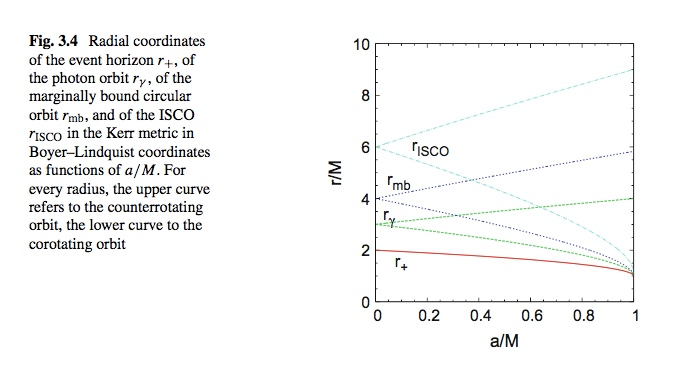
\includegraphics[scale=0.4] {figures/kerrradii.jpeg}
      \end{figure}
	\end{center}	
\end{frame}


\section{Geodesics in Kerr Spacetime}    
\begin{darkframes}

\subsection{Hamilton-Jacobi Formulation}
\begin{frame}
\Huge
Hamilton-Jacobi Formulation
\end{frame}

\begin{frame}{Hamilton-Jacobi Formulation}
    \[ \mathcal{L} = \frac{1}{2}  g_{\mu\nu} \dot{x}^\mu \dot{x}^\nu \]
    \pause
    \[ p_\mu = \frac{\partial \mathcal{L}}{\partial \dot{x}^\mu} =  g_{\mu\nu} \dot{x}^\nu \]
    \pause
    \[ \mathcal{H} = \frac{1}{2}  g^{\mu\nu} p_\mu p_\nu \]
\end{frame}

\begin{frame}{Hamilton-Jacobi Formulation}
    Hamilton's principal function
    \[ S = S \left( x^\mu ; \lambda \right)\]
    \pause
    \[ p_\mu = \frac{\partial S}{\partial x^\mu} \]
    \pause
    Hamilton-Jacobi Equation
    \pause
    \[  \frac{1}{2}  g^{\mu\nu} \frac{\partial S}{\partial x^\mu} \frac{\partial S}{\partial x^\nu} - \frac{\partial S}{\partial \lambda} =0 \]
\end{frame}

\begin{frame}{Kerr's Solution}
    	Boyer-Lindquist coordinates: $\left(t,r,\theta,\varphi\right)$
     	\begin{align*}
            ds^{2} &= -\frac{\Delta-a^{2}\sin^{2}\theta}{\varrho}dt^{2}-\left(\frac{r^{2}+a^{2}-\Delta}{\varrho}\right)2a\sin^{2}\theta dtd\varphi\nonumber \\
             & +\frac{\varrho}{\Delta}dr^{2}+\varrho d\theta^{2}+\left(\frac{\left(r^{2}+a^{2}\right)^{2}-\Delta a^{2}\sin^{2}\theta}{\varrho}\right)\sin^{2}\theta d\varphi^{2}.
      	\end{align*}
     	\pause
   	$$\varrho  = r^{2}+a^{2}\cos^{2}\theta$$
    $$\Delta =  r^{2}-2Mr+a^{2}$$
\end{frame}

\begin{frame}{Kerr's Solution}
     	\begin{align*}
            \left( \frac{\partial}{\partial s} \right)^{2} = &- \frac{A}{\varrho \Delta} \left( \frac{\partial}{\partial t} \right)^{2} - \frac{4aMr}{\varrho \Delta} \left( \frac{\partial}{\partial t} \right) \left( \frac{\partial}{\partial \varphi} \right) +\frac{\Delta}{\varrho}\left( \frac{\partial}{\partial r} \right)^2 \nonumber \\
             & + \frac{1}{\varrho} \left( \frac{\partial}{\partial \theta} \right)^{2} + \frac{\Delta - a^2 \sin^2 \theta}{\varrho \Delta \sin^{2}\theta} \left( \frac{\partial}{\partial \varphi} \right)^{2}
      	\end{align*}
    \pause
    $$A = (r^2 + a^2)^2 -a^2 \Delta \sin^2 \theta$$ 	
   	$$\varrho  = r^{2}+a^{2}\cos^{2}\theta$$
    $$\Delta =  r^{2}-2Mr+a^{2}$$
\end{frame}

\begin{frame}{Hamilton-Jacobi Formulation}
    Hamilton-Jacobi Equation
     \[ 2 \frac{\partial S}{\partial \lambda}  = g^{\mu\nu} \frac{\partial S}{\partial x^\mu} \frac{\partial S}{\partial x^\nu} \]
    \pause
    \begin{align*}
           2 \frac{\partial S}{\partial \lambda} = &- \frac{A}{\varrho \Delta} \left( \frac{\partial S}{\partial t} \right)^2 - \frac{4aMr}{\varrho \Delta} \left( \frac{\partial S}{\partial t} \right) \left( \frac{\partial S}{\partial \varphi} \right) +\frac{\Delta}{\varrho}\left( \frac{\partial S}{\partial r} \right)^2 \nonumber \\
             & + \frac{1}{\varrho} \left( \frac{\partial S}{\partial \theta} \right)^{2} + \frac{\Delta - a^2 \sin^2 \theta}{\varrho \Delta \sin^{2}\theta} \left( \frac{\partial S}{\partial \varphi} \right)^{2}
    \end{align*}   
\end{frame}

\begin{frame}{Hamilton-Jacobi Formulation}
    Hamilton Principal Function
    \[S = \frac{1}{2} \lambda \delta -\varepsilon t +\ell_z \varphi + S_r (\theta) + S_\theta (\theta)\]
	Separation of the Hamilton-Jacobi Equation. Carter Constant
	\begin{align*}
	&\Delta \left( \frac{dS_r}{dr}\right)^2 - \frac{1}{\Delta} \left[ (r^2 +a^2) \varepsilon - a \ell_z \right]^2 + (\ell_z - a \varepsilon)^2 + \delta r^2  =\\
	& -\left( \frac{dS_\theta}{d\theta}\right)^2 - \left(\frac{\ell_z^2}{\sin^2 \theta} - a^2 \varepsilon^2 + \delta a^2 \right)\cos^2 \theta = \mathcal{C}
	\end{align*}      
\end{frame}

\begin{frame}{Hamilton-Jacobi Formulation}
	Separation of the Hamilton-Jacobi Equation. Carter Constant
	\begin{align*}
	\Delta \left( \frac{dS_r}{dr}\right)^2 &= \frac{1}{\Delta} \left[ (r^2 +a^2) \varepsilon - a \ell_z \right]^2 - \left[ \mathcal{C} + (\ell_z - a \varepsilon)^2 + \delta r^2 \right]\\ 
	\left( \frac{dS_\theta}{d\theta}\right)^2 &= \mathcal{C} - \left( \frac{\ell_z^2}{\sin^2 \theta} - a^2 \varepsilon^2 + \delta a^2 \right) \cos^2 \theta	
	\end{align*}      
\end{frame}

\begin{frame}{Hamilton-Jacobi Formulation}
	\begin{align*}
	S_r &= \int \frac{\sqrt{R(r')}}{\Delta}dr'\\
	S_\theta &= \int \sqrt{\Theta(\theta')}d\theta'
	\end{align*}
	\pause 
	\begin{align*}
	R(r) &= \left[ (r^2 +a^2) \varepsilon - a \ell_z \right]^2 - \Delta \left[\mathcal{C} + (\ell_z - a \varepsilon)^2 + \delta r^2 \right]\\
	\Theta(\theta) &= \mathcal{C} - \left[ \frac{\ell_z^2}{\sin^2 \theta} + a^2 \left(\delta - \varepsilon^2 \right) \right] \cos^2 \theta
	\end{align*}      
\end{frame}

\begin{frame}{Carter Constant}
	\[\left( \frac{dS_\theta}{d\theta}\right)^2 = \mathcal{C} - \left( \frac{\ell_z^2}{\sin^2 \theta} - a^2 \varepsilon^2 + \delta a^2 \right) \cos^2 \theta\] 
	\bigskip
	\pause
	
	\[ \mathcal{C} = p_\theta^2 + p_\varphi^2 \cot^2 \theta + a^2 (\delta - \varepsilon^2) \cos^2 \theta \]     
\end{frame}

\begin{frame}{Carter Constant}
	Schwarzschild:		
	\[ \mathcal{C} = \left( p_\theta^2 + \frac{p_\varphi^2}{\sin^2 \theta} \right) - p_\varphi^2 = \ell^2 - \ell_z^2 \]   
	where $\ell = p_\theta^2 + \frac{p_\varphi^2}{\sin^2 \theta}$ is the total angular momentum.
\end{frame}

\begin{frame}{Carter Constant}
	Kerr:
	\pause		
	\begin{itemize}
	\item $\mathcal{C}$ has not a direct physical interpretation.
	\item $\mathcal{C}=0$ implies that the motion is in the equatorial plane.
	\end{itemize}
\end{frame}



\subsection{Equations of Motion}
\begin{frame}
	\huge
    {Equations of Motion}
\end{frame}

\begin{frame}{Equations of Motion}
    Hamilton Canonical Equations
    \pause
    \[ \dot{x}^\mu = p^\mu = g^{\mu \nu} p_\nu = g^{\mu\nu} \frac{\partial S}{ x^\nu} \]
\end{frame}

\begin{frame}{Equations of Motion}
    \footnotesize

    \begin{align*}
    \varrho^2 \dot{r}^2 &= R \\
    \varrho^2 \dot{\theta}^2 &= \Theta \\
    \varrho \dot{\varphi} &= \frac{1}{\Delta} \left[ 2aMr\varepsilon + (\varrho - 2Mr)\frac{\ell_z}{\sin^2 \theta} \right] \\
    \varrho \dot{t} &= \frac{1}{\Delta} \left[ A\varepsilon + 2aMr \ell_z \right]
    \end{align*}
    \pause
    \begin{align*}
    R(r) &= \left[ (r^2 +a^2) \varepsilon - a \ell_z \right]^2 - \Delta \left[\mathcal{C} + (\ell_z - a \varepsilon)^2 + \delta r^2 \right]\\
	\Theta(\theta) &= \mathcal{C} - \left[ \frac{\ell_z^2}{\sin^2 \theta} + a^2 \left(\delta - \varepsilon^2 \right) \right] \cos^2 \theta\\
    A &= (r^2 + a^2)^2 - a^2 \Delta \sin^2 \theta \\
    \varrho  &= r^{2}+a^{2}\cos^{2}\theta \\
    \Delta &= r^{2}-2Mr+a^{2} 
    \end{align*}
\end{frame}

\subsection{Imaging a Black Hole}
\begin{frame}
	\huge
    {Imaging a Black Hole}
\end{frame}

\begin{frame}
	\huge
    {Image Plane of a Distant Observer}
\end{frame}

\begin{frame}{Image Plane of a Distant Observer}
    \begin{itemize}
    \item A distant observer receives the electromagnetic radiation from the accretion disk, around the black hole.
    \pause
    \item It is usual to define a plane of observation and consider the photons with momentum orthogonal to the plane. These photons' trajectories are integrated backwards in time to find the position of the emission point in the disk.
    \end{itemize}
\end{frame}

\end{darkframes}
\begin{frame}{Image Plane of a Distant Observer}
	\begin{center}
      \begin{figure}
      	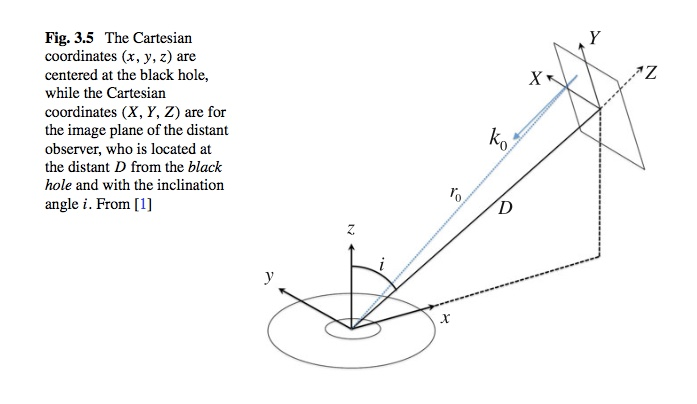
\includegraphics[scale=0.35] {figures/diskobservation.jpeg}
      \end{figure}
	\end{center}	
\end{frame}

\begin{darkframes}

\begin{frame}{Coordinate Systems}
    \begin{itemize}
    \item $(X,Y,Z)$: Cartesian coordinates in the image plane
    \pause
    \item $(x,y,z)$: Cartesian coordinates centered at the black hole.
    \pause
    \item $i$: Inclination angle of the observer with respect to the $z$ direction.
    \pause
    \item $D$: Distance observer-black hole.
    \end{itemize}
\end{frame}

\begin{frame}{Coordinate transformations}
	\begin{align*}
    x &= D\sin i - Y \cos i + Z\sin i\\
    y &= X\\
    z &= D\cos i + Y \sin i + Z\cos i
    \end{align*}
    
    \begin{align*}
    r &= \sqrt{x^2 + y^2 + z^2}\\
    \theta &= \arccos \left( \frac{z}{r} \right)\\
    \varphi &= \arctan \left( \frac{z}{r} \right)
    \end{align*}
\end{frame}

\begin{frame}
	\huge
    {Photon Trajectory Tracing}
\end{frame}

\begin{frame}{Photon Trajectory Tracing}
	Consider a photon received at $(X_0,Y_0,0)$ with 3-momentum $\textbf{k}_0 = -k_0 \hat{Z}$, i.e. perpendicular to the observer plane.\\
	
	The initial conditions for the position of the photon (to trace back the trajectory), as seen from the black hole and in spherical coordinates, are
    \begin{align*}
	t_0 &= 0\\     
    r_0 &= \sqrt{X_0^2 + Y_0^2 + D^2}\\
    \theta_0 &= \arccos \left( \frac{Y_0 \sin i + D \cos i}{r_0} \right)\\
    \varphi_0 &= \arctan \left( \frac{X_0}{D \sin i - Y_0 \cos i} \right)
    \end{align*}
\end{frame}

\begin{frame}{Photon Trajectory Tracing}
	The initial conditions for the 4-momentum of the photon $k^\mu$ (to trace back the trajectory), as seen from the black hole and in spherical coordinates, are calculated with the transformation law,
	\[ k^\mu = \frac{\partial x^\mu}{\partial \bar{x}^\alpha} \bar{k}^\alpha \]
	\pause
	\footnotesize
    \begin{align*}
	k_0^r &= -\frac{D}{r} k_0\\     
    k_0^\theta &= \frac{\cos i - (Y_0 \sin i + D \cos i)\frac{D}{r_0^2} }{\sqrt{X_0^2 + (D \sin i - Y_0 \cos i)^2}} k_0\\
    k_0^\varphi &= \frac{X_0 \sin i}{X_0^2 + (D \sin i - Y_0 \cos i)^2} k_0
    \end{align*}
\end{frame}

\begin{frame}{Photon Trajectory Tracing}
	The $k^t_0$ component of the initial 4-momentum is calculated by the condition $g_{\mu\nu} g^\mu k`^\nu = 0 $,
	\[ k_0 ^t = \sqrt{(k_0^r)^2 + r_0^2 (k_0^\theta)^2 + r_0^2 \sin^2 \theta_0 (k_0^\varphi)^2}\]
\end{frame}

\begin{frame}{Photon Trajectory Tracing}
	Given the initial conditions for position and momentum, it is possible to trace  the trajectory of any photon in the observer plane back to the accretion disk.
\end{frame}

\begin{frame}
	\huge
    {Non-Coordinate Basis}
\end{frame}

\begin{frame}{Tetrads}
	Introduce a non-coordinate basis or orthonormal tetrad,
	\pause
	\begin{align*}
	\textbf{E}_{(a)} &= E_{(a)}^\mu \partial_\mu \\
	\textbf{E}^{(a)} &= E^{(a)}_\mu dx^\mu,
	\end{align*}
	subject to the conditions
	\begin{align*}
	\eta_{(a)(b)} &= E_{(a)}^\mu E_{(b)}^\nu g_{\mu\nu} \\
	\eta^{(a)(b)} &= E^{(a)}_\mu E^{(b)}_\nu g{\mu\nu}
	\end{align*}
	and $ det |E_{(a)^\mu} | >0$ (to preserve the orientation).
\end{frame}

\begin{frame}{Tetrads}
	Components of a vector in the orthonormal tetrad basis,
	\pause
	\begin{align*}
	V^{(a)} &= E^{(a)}_\mu V^\mu \\
	V_{(a)} &= E_{(a)}^\mu V_\mu
	\end{align*}
\end{frame}

\begin{frame}{General Metric}
	Consider a general stationary, axisymmetric, asymptotically flat metric
	\[ ds^2 = -e^{2\alpha(r)}dt^2 + e^{2\beta(r)} dr^2 + e^{2\gamma(r,\theta)} d\theta^2 + e^{2\epsilon(r,\theta)} (d\varphi-\omega dt)^2\] 
	\pause
	We identify the \textit{locally non-rotating observers} as those whose world-lines have 
	\pause
	\begin{align*}
	r &= \textrm{constant} \\
	\theta &= \textrm{constant}\\
	\varphi &= \omega t+\textrm{constant}
	\end{align*}
\end{frame}

\begin{frame}{General Metric}
	The non-coordinate basis of the locally non-rotating observers is given by the tetrad
	\begin{align*}
	E^\mu _{(t)} &= \left( e^{-\beta}, 0, 0, \omega e^{-\beta} \right)\\
	E^\mu _{(r)} &= \left( 0, e^{-\alpha}, 0, 0 \right)\\
	E^\mu _{(\theta )} &= \left( 0, 0, e^{-\gamma}, 0 \right)\\
	E^\mu _{(\varphi )} &= \left( 0, 0, 0, e^{-\epsilon} \right)
	\end{align*}
\end{frame}

\begin{frame}{General Metric}
	and the dual basis,	
	\begin{align*}
	E_\mu ^{(t)} &= \left( e^{\beta}, 0, 0, 0 \right)\\
	E_\mu ^{(r)} &= \left( 0, e^{\alpha}, 0, 0 \right)\\
	E_\mu ^{(\theta )} &= \left( 0, 0, e^{\gamma}, 0 \right)\\
	E_\mu ^{(\varphi )} &= \left( -\omega e^{\epsilon}, 0, 0, e^{\epsilon} \right)
	\end{align*}
\end{frame}

\begin{frame}{Kerr Metric}
	For the particular case of the Kerr metric the tetrad describing 	the non-coordinate basis of the locally non-rotating observers is
	\begin{align*}
	E^\mu _{(t)} &= \left( \sqrt{\frac{A}{\varrho \Delta}}, 0, 0, \frac{2Mar}{\sqrt{A \varrho \Delta}} \right)\\
	E^\mu _{(r)} &= \left( 0, \sqrt{\frac{\Delta}{\varrho}}, 0, 0 \right)\\
	E^\mu _{(\theta )} &= \left( 0, 0, \frac{1}{\sqrt{\varrho}}, 0 \right)\\
	E^\mu _{(\varphi )} &= \left( 0, 0, 0, \frac{1}{\sin \theta}\sqrt{\frac{\varrho}{A}} \right)
	\end{align*}
\end{frame}

\begin{frame}{Kerr Metric}
	and the dual basis is
	\begin{align*}
	E_\mu ^{(t)} &= \left( \sqrt{\frac{\varrho \Delta}{A}}, 0, 0, 0 \right)\\
	E_\mu ^{(r)} &= \left( 0, \sqrt{\frac{\varrho}{\Delta}}, 0, 0 \right)\\
	E_\mu ^{(\theta )} &= \left( 0, 0, \sqrt{\varrho}, 0 \right)\\
	E_\mu ^{(\varphi )} &= \left( -\frac{2Mar \sin \theta}{\sqrt{\varrho A}}, 0, 0, \sqrt{\frac{A}{\varrho}} \sin \theta \right)
	\end{align*}
\end{frame}

\begin{frame}{Momentum Components in the Non-Coordinate Basis}
	The momentum components of a particle moving in Kerr's spacetime are
	\[ p_\mu = \frac{\partial S}{\partial x^\mu} \]
	\pause
	\begin{align*}
	p_t &= -\varepsilon\\
	p_r &= \frac{\sqrt{R}}{\Delta}\\
	p_\theta &= \sqrt{\Theta}\\
	p_\varphi &= \ell_z
	\end{align*}
\end{frame}

\begin{frame}{Momentum Components in the Non-Coordinate Basis}
	In the non-coordinate basis, the momentum components of a particle are
	\[ p^{(a)} = E^{(a)}_\mu p^\mu = \eta ^{(a)(b)} E_{(b)}^\mu p_\mu  \]
	\pause
	\begin{align*}
	p^(t) &= -E_{(t)}^\mu p_\mu\\
	p^r &= E_{(r)}^\mu p_\mu\\
	p^\theta &= E_{(\theta)}^\mu p_\mu\\
	p^\varphi &= E_{(\varphi)}^\mu p_\mu
	\end{align*}
\end{frame}

\begin{frame}
	\huge
    {Celestial Coordinates}
\end{frame}

\begin{frame}{Celestial Coordinates}
	The position of a photon in the image plane of the distant observer is given by the coordinates 
	\[\begin{cases}
	X_0 &= \alpha = \lim_{r\rightarrow\infty} \left( \frac{rp^{(\varphi)}}{p^{(t)}} \right) \\
	Y_0 &= \beta = \lim_{r\rightarrow\infty} \left( \frac{rp^{(\theta)}}{p^{(t)}} \right)
	\end{cases}\]
\end{frame}

\begin{frame}{Celestial Coordinates}
	\[\begin{cases}
	\alpha &= -\xi \csc i\\	
	\beta &= \pm \sqrt{\eta + a^2 \cos^2 i - \xi^2 \cot^2 i}
	\end{cases}\]
	\pause
	\[\begin{cases}
    \xi &= \frac{\ell_z}{\varepsilon}\\
    \eta &= \frac{\mathcal{C}}{\varepsilon^2}
	\end{cases}\]
\end{frame}


\begin{frame}
	\huge
    {Black Hole's Shadow}
\end{frame}

\begin{frame}{Effective Potential for Photons}
    \begin{align*}
    R(r) &= \left[ (r^2 +a^2) \varepsilon - a \ell_z \right]^2 - \Delta \left[\mathcal{C} + (\ell_z - a \varepsilon)^2 + \delta r^2 \right]\\
	\Theta(\theta) &= \mathcal{C} - \left[ \frac{\ell_z^2}{\sin^2 \theta} + a^2 \left(\delta - \varepsilon^2 \right) \right] \cos^2 \theta
    \end{align*}
    \pause
    Consider these expressions for photons, $\delta=0$, and using the quantities
    \[\begin{cases}
    \xi &= \frac{\ell_z}{\varepsilon}\\
    \eta &= \frac{\mathcal{C}}{\varepsilon^2}
	\end{cases}\]    
\end{frame}

\begin{frame}{Effective Potential for Photons}
    \begin{align*}
    R(r) &= \left[ r^2 +a^2  - a \xi  \right]^2 \varepsilon^2- \Delta \left[\eta + (\xi - a )^2 \right]\varepsilon^2\\
	\Theta(\theta) &= \eta \varepsilon^2   - \left[ \frac{\xi^2}{\sin^2 \theta} - a^2 \right] \varepsilon^2 \cos^2 \theta
    \end{align*}
  
\end{frame}

\begin{frame}{Effective Potential for Photons}
	\begin{align*}
	\mathcal{R}(r) &= \frac{R(r)}{\varepsilon^2} = \left[ r^2 +a^2  - a \xi  \right]^2 - \Delta \left[\eta + (\xi - a )^2 \right] \\
	\vartheta (\theta) &= \frac{\Theta(\theta)}{\varepsilon^2} = \left[\eta + (\xi - a )^2 \right] - \left[ a \sin \theta - \xi \csc \theta \right]^2
	\end{align*} 
	\pause 
	\[\Delta = r^{2}-2Mr+a^{2} \] 
\end{frame}

\begin{frame}{Equations of Motion for Photons}
	\begin{align*}
    \varrho^2 \dot{r}^2 &= \mathcal{R} \\
    \varrho^2 \dot{\theta}^2 &= \vartheta \\
    \varrho \dot{\varphi} &= \frac{1}{\Delta} \left[ 2aMr + \frac{\xi (\varrho - 2Mr)}{\sin^2 \theta} \right] \\
    \varrho \dot{t} &= \frac{1}{\Delta} \left[ A + 2aMr \xi \right]
    \end{align*}
\end{frame}

\begin{frame}{Photon Sphere}
	Circular motion of photons: $\dot{r} = 0$
	\pause
	\[\begin{cases}
	\mathcal{R} &= 0\\
	\partial_r \mathcal{R} &= 0
	\end{cases}\]
\end{frame}

\begin{frame}{Photon Sphere}
	Solving for $\xi$ and $\eta$ we obtain these quantities for the circular orbit as functions of the parameter $r$,
	\pause
	\begin{align*}
	\xi_{c} &= \frac{M(r^2 -a^2) - r \Delta}{a(r-M)} \\
	\eta_{c} &= \frac{r^3 \left[ 4M\Delta - r (r-M)^2\right]}{a^2(r-M)^2}
	\end{align*}
\end{frame}

\begin{frame}{Photon Sphere}
	There are three possible cases regarding the stability of circular orbits of photons
	\pause
	\begin{enumerate}
	\item If $\partial_r^2 \mathcal{R} > 0$ : Stable circular orbits
	\pause
	\item If $\partial_r^2 \mathcal{R} < 0$ : Unstable circular orbits. The photon straddles the boundary between two regions: $\partial_r \mathcal{R} = 0$; if perturbed one way it falls into the horizon, if perturbed the other way it flies outwards.
	\pause
	\item If $\partial_r^2 \mathcal{R} = 0$ : Marginally stable circular orbit (Photon Sphere). $r=r_{ps}$.
	\end{enumerate}	 
\end{frame}

\begin{frame}{Black Hole's Shadow}
	\begin{align*}
	\alpha &= -\xi_c \csc i\\	
	\beta &= \sqrt{\eta_c + a^2 \cos^2 i - \xi_c^2 \cot^2 i}
	\end{align*}
	\pause
	\begin{align*}
	\xi_c &= \frac{M(r^2 -a^2) - r \Delta}{a(r-M)} \\
	\eta_c &= \frac{r^3 \left[ 4M\Delta - r (r-M)^2\right]}{a^2(r-M)^2}
	\end{align*}
\end{frame}

\begin{frame}{Black Hole's Shadow}
	Schwarzschild's Black Hole:	
	\[ \alpha^2 + \beta^2 = R_{shadow}^2\]
	\pause
	\[ R_{shadow} = \sqrt{27 M^2} \]
\end{frame}

\begin{frame}{Shadow of Sagittarius A*}
	$M_{SgrA*} = 4 \times 10^6 M_\odot\ $\\
	\bigskip
	\pause
	$r_H = 2 M = \frac{2GM}{c^2}$\\
	\pause
	$r_H = 1.2 \times 10^{10} \textrm{ m.} = 1.2 \times 10^{7} \textrm{ km.}$ \\
	\pause
	$r_H = 0.1 \textrm{ AU} $\\
	\bigskip
	\pause
	$R_{shadow} = \sqrt{27 M^2} = 3 \sqrt{3} M$\\
	\pause
	$R_{shadow} = 3 \sqrt{3} \frac{GM}{c^2} = 3 \times 10^{10} \textrm{ m.}$ \\
	\pause
	$R_{shadow} = 3 \times 10^{7} \textrm{ km.} = 0.2 \textrm{ AU} $ \\
\end{frame}

\begin{frame}{Shadow of Sagittarius A*}
	$R_{shadow} = 0.2 \textrm{ AU} = 9.7 \times 10^{-10} \textrm{ kpc}$ \\
	\bigskip
	\pause
	$D = 8 \textrm{ kpc} $\\
	\bigskip
	$\theta_{shadow} = \frac{R_{shadow}}{D}$\\
	\pause
	$\theta_{shadow} = 1.2 \times 10^{-11} \textrm{ rad}$\\
	\pause
	$\theta_{shadow} = 2.5$ $\mu$arcsec
\end{frame}

\begin{frame}{Shadow of Sagittarius A*}
	Very Long Baseline Interferometry (VLBI)\\
	\bigskip	
	\pause
	$\theta_{res} \sim \frac{\lambda}{d}$\\
	\bigskip
	\pause
	$\lambda \sim 1 \textrm{ mm}$\\
	\pause
	$d \sim 10^3 \textrm{ km}$\\
	\bigskip
	\pause
	$\theta_{res} \sim 10$ $\mu$arcsec	
\end{frame}

\begin{frame}{Next Lecture}
  	\Large
	{08. Accretion}
\end{frame}






\begin{frame}
	\Large
	{Alternative derivation of the Celestial Coordinates}
\end{frame}

\begin{frame}{Celestial Coordinates}
    \begin{itemize}
    \item A distant observer receives the electromagnetic radiation from the surroundings of the black hole.
    \pause
    \item Let the observer be at $r\rightarrow \infty$  with inclination angle $i$ (between the rotation axis of the black hole and the observer's line of sight).
    \pause
    \item The celestial coordinates $(\alpha, \beta )$ are the apparent angular distances of the image on the celestial sphere measured by the observer.
    \end{itemize}
\end{frame}

\begin{frame}{Celestial Coordinates}
	\begin{itemize}
	\item The distant observer may set up a euclidean coordinate system $(x,y,z)$ with the black hole at the origin and its rotation axis along $z$.
	\pause
	\item Using the Boyer-Lindquist coordinates describing the black hole, the observer will be located at some coordinates $(r_0, \theta_0, \varphi_0)$, with  $r_0$ very large.
    	\end{itemize}
\end{frame}

\end{darkframes}

\begin{frame}{Celestial Coordinates}
	\begin{center}
      \begin{figure}
      	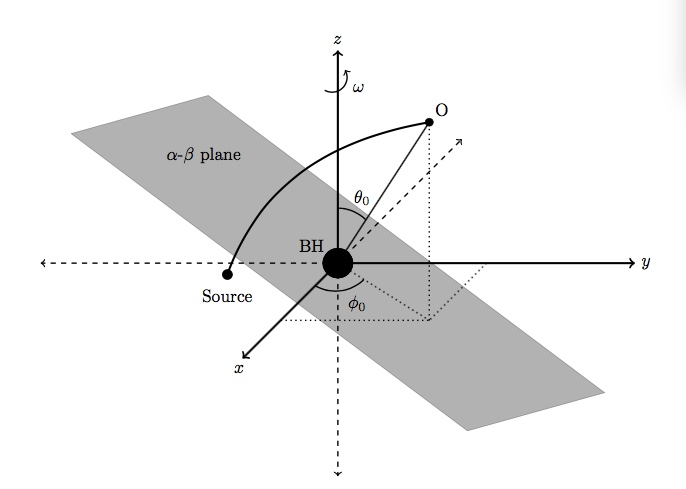
\includegraphics[scale=0.35] {figures/celestialcoordinates1.jpeg}
      \end{figure}
	\end{center}	
\end{frame}

\begin{darkframes}

\begin{frame}{Celestial Coordinates}
	\begin{itemize}
	\item Note that the inclination angle is precisely $\theta_0 = i$. Hence the position of the observer is $(r_0, i, \varphi_0)$
	\pause
	\item Without loosing generality, we rotate the $(x,y,z)$ system so that the angular position of the observer in the Boyer-Lindquist coordinates is $\varphi_0 = 0$. 
	\pause
	\item The position of the observer becomes $(r_0, i, 0)$
	\pause
	\item Then, the observer lies in the $x-z$ plane while the $y$-axis lies in the $(\alpha, \beta)$ plane (remember that the observer plane is perpendicular to the line of sight).  	 
    	\end{itemize}
\end{frame}

\end{darkframes}

\begin{frame}{Celestial Coordinates}
	\begin{center}
      \begin{figure}
      	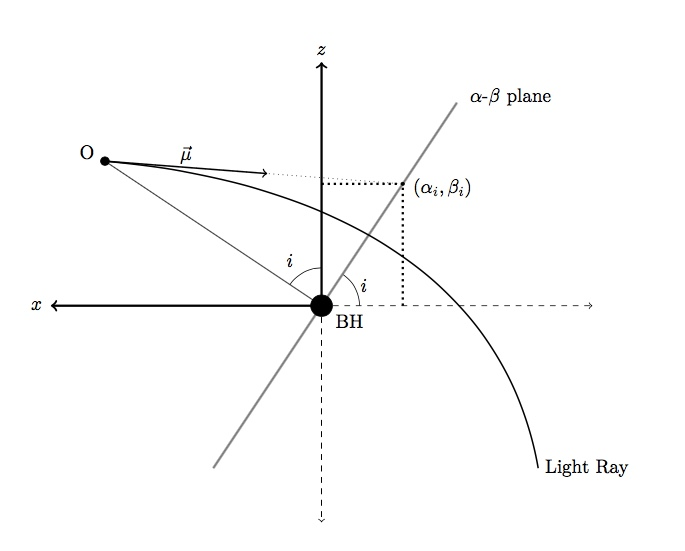
\includegraphics[scale=0.35] {figures/celestialcoordinates2.jpeg}
      \end{figure}
	\end{center}	
\end{frame}

\begin{darkframes}

\begin{frame}{Trajectory of a Light Ray}
	In the observer's reference frame, an incoming light ray trajectory may be decribed by a parametric curve
	\[ \begin{cases}
	X = X(r)\\
	Y = Y(r)\\
	Z = Z(r)\\
	\end{cases} \] 
	such that
	\[ r^2 = X^2 (r) + Y^2 (r) + Z^2 (r) \]	 
\end{frame}	

\begin{frame}{Trajectory of a Light Ray}
	The tangent vector to this parametric curve at the observer's location is
	\[ \vec{\mu} = (\mu_1, \mu_2, \mu_3) = \left( \left. \frac{dX}{dr}\right|_{r_0}, \left. \frac{dY}{dr} \right|_{r_0}, \left. \frac{dZ}{dr} \right|_{r_0} \right) \]	 
\end{frame}
	
\begin{frame}{Trajectory of a Light Ray}
	From the point of view of the observer, this tangent vector defines the trajectory of the photon as a straight line which intersects the observer's celestial plane at the coordinates $(\alpha_i, \beta_i)$ and can be written parametrically as
	\[ \frac{x-x_0}{\mu_1} = \frac{y-y_0}{\mu_2} = \frac{z-z_0}{\mu_3}\]
\end{frame}

\begin{frame}{Trajectory of a Light Ray}
$(x_0, y_0, z_0)$ are the coordinates of the observer's position.\\
\pause
This can be written as
\[ (x_0, y_0, z_0) = (r_0 \sin i, 0, r_0 \cos i)\]	
\pause
The celestial coordinates $(\alpha_i, \beta_i)$ can be written as
\[ (\alpha_i, \beta_i) = (x_i, y_i, z_i) = (-\beta_i \cos i, \alpha_i, \beta_i \sin i)\]
\end{frame}

\begin{frame}{Trajectory of a Light Ray}
	\[ \frac{x-x_0}{\mu_1} = \frac{y-y_0}{\mu_2} = \frac{z-z_0}{\mu_3}\]
	\pause
	\[ \frac{-\beta_i \cos i-r_0 \sin i}{\mu_1} = \frac{\alpha_i}{\mu_2} = \frac{\beta_i \sin i-r_0 \cos i}{\mu_3}\]
\end{frame}

\begin{frame}{Trajectory of a Light Ray}
	Using the transformation between cartesian and spherical coordinates,
	\footnotesize
	\begin{align*}
	X(r) &= r \sin \theta \cos \varphi\\
	Y(r) &= r \sin \theta \sin \varphi\\
	Z(r) &= r \cos \theta,
	\end{align*}
	\normalsize
	we obtain the components of $\vec{\mu}$,
	\footnotesize
	\begin{align*}
	\mu_1 &=  \left. \frac{dX}{dr}\right|_{r_0} = \sin i + r_0 \cos i \left. \frac{d \theta}{dr}\right|_{r_0}\\
	\mu_2 &=  \left. \frac{dY}{dr}\right|_{r_0} = r_0 \sin i \left. \frac{d \varphi}{dr}\right|_{r_0}\\
	\mu_3 &=  \left. \frac{dZ}{dr}\right|_{r_0} = \cos i - r_0 \sin i \left. \frac{d \theta}{dr}\right|_{r_0}
	\end{align*}
\end{frame}

\begin{frame}{Trajectory of a Light Ray}
	\[ \frac{-\beta_i \cos i-r_0 \sin i}{\mu_1} = \frac{\alpha_i}{\mu_2} = \frac{\beta_i \sin i-r_0 \cos i}{\mu_3}\]
	\bigskip
	\pause
	\[ \frac{-\beta_i \cos i-r_0 \sin i}{\sin i + r_0 \cos i \left. \frac{d \theta}{dr}\right|_{r_0}} = \frac{\alpha_i}{r_0 \sin i \left. \frac{d \varphi}{dr}\right|_{r_0}} = \frac{\beta_i \sin i-r_0 \cos i}{\cos i - r_0 \sin i \left. \frac{d \theta}{dr}\right|_{r_0}}\]
\end{frame}

\begin{frame}{Celestial Coordinates}
	\begin{align*}
	\alpha_i &= \lim_{r_0 \rightarrow \infty} -r_0^2 \sin^2 \theta_0 \left. \frac{d\varphi}{dr}\right|_{r_0}\\	
	\beta_i &= \lim_{r_0 \rightarrow \infty} r_0^2 \left. \frac{d\theta}{dr}\right|_{r_0}
	\end{align*}
\end{frame}

\begin{frame}{Celestial Coordinates}
Using the equations of motion for the photons, we obtain
	\begin{align*}
	\alpha_i &= -\xi \csc i\\	
	\beta_i &= \sqrt{\eta + a^2 \cos^2 i - \xi^2 \cot^2 i}
	\end{align*}
\end{frame}

  
  \end{darkframes}
\end{document}
